\documentclass{standalone}
\usepackage{tikz, pgfplots, amssymb, amsmath, amsfonts}
\newcommand{\vect}[1]{\boldsymbol{\mathbf{#1}}}
\usepgfplotslibrary{fillbetween}
\pgfplotsset{compat=1.18}
\begin{document}
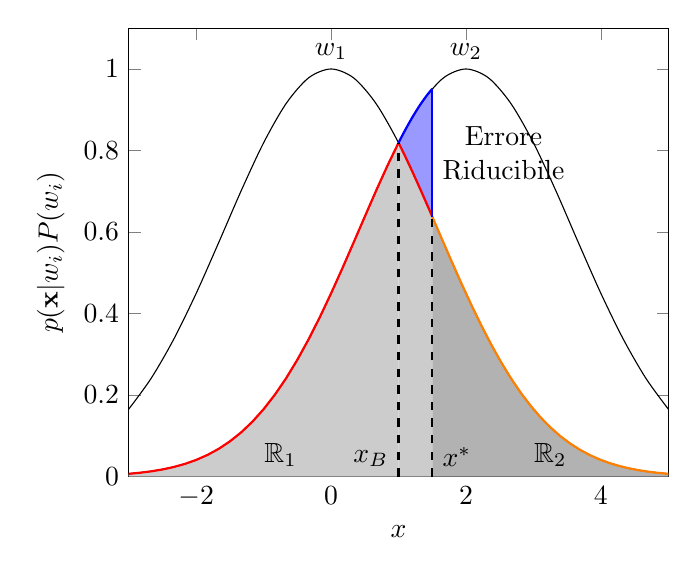
\begin{tikzpicture}
\begin{axis}[
    xlabel=$x$,
    ylabel=$p(\vect{x}|w_i)P(w_i)$,
    ymin=0, 
    xmin=-3,xmax=5,
    ]
    \addplot[smooth, domain=-3:5]
        {exp(-1/5*x^2)};
    \addplot[smooth, domain=-3:5]
        {exp(-1/5*(x-2)^2)};
    
    \addplot[solid, thick, red, domain=-3:1, name path=A]
        {exp(-1/5*(x-2)^2)};
    \addplot[solid, thick, red, domain=1:1.5, name path=B]
        {exp(-1/5*x^2)};
    \addplot[draw=none,name path=C] {0};
    \addplot[gray!40]fill between[of=A and C, soft clip={domain=-3:1}];
    \addplot[gray!40]fill between[of=B and C, soft clip={domain=1:1.5}];
    
    
    \addplot[solid, thick, orange, domain=1.5:5, name path=D]
        {exp(-1/5*x^2)};
    \addplot[solid, thick, blue, domain=1:1.5, name path=E]
        {exp(-1/5*(x-2)^2)};
        
    \addplot[darkgray!40]fill between[of=D and C, soft clip={domain=1.5:5}];
    \addplot[blue!40]fill between[of=E and B, soft clip={domain=1:1.5}];
    

    \draw
        (0,1)node[above]{$w_1$}
        (2,1)node[above]{$w_2$}
    ;
    \draw[dashed, thick]
        (1,0)node[above left]{$x_B$}--(1,0.8187)
        (1.5,0)node[above right]{$x^*$}--(1.5,0.637)
    ;
    \draw[thick, blue](1.5,0.637)--(1.5,0.95)node[color=black, midway, right, align=center]{Errore\\Riducibile};
    \draw[draw=none](-3,0)--(1.5,0)node[midway, above, color=black,]{$\mathbb{R}_1$};
    \draw[draw=none](1.5,0)--(5,0)node[midway, above, color=black,]{$\mathbb{R}_2$};
\end{axis}
\end{tikzpicture}
\end{document}